\begin{abstract}
Self-evolving agents increasingly store reusable skills as persistent, named objects that are selected, credited, updated, and sometimes retired across rounds. We ask a representation question that precedes optimizer design: if one semantic skill is replaced by several exact-content identities, should the agent's future evolution change? We identify two independent ways in which it can. First, identity-indexed selection can duplicate semantic mass. Second, and more subtly, the same identities can serve as persistent evidence buckets: identical post-selection feedback is fragmented before a nonlinear lifecycle gate. In released Skill Self-Play (Skill-SP) code, eight identical retirement-eligible records retire one canonical skill, while an exact two-way split receives four records per identity and leaves the semantic class active; aggregating credit at the semantic quotient restores the canonical decision. We derive an exact phase law: for a per-identity threshold $M$, balanced $k$-way refinement creates a fragmentation window $M\le N<kM$ and retirement lag $(k-1)M$, verified with zero mismatches over 882 released-controller configurations. A $2\times2$ intervention separates selection from credit: quotienting either surface alone leaves the other defect, while quotienting both restores both canonical semantic endpoints. SkillsVote independently exhibits the same partition-before-update request topology. We retain earlier target-realizability analysis as the general partial-overlap selection channel and explicitly bound the result: Skill-SP's evolved runtime states are not released, and a preregistered AutoSkill heldout pilot blocks task-general behavioral claims. The resulting view is that skill identity can be both an action coordinate and a persistent learning-state coordinate; representation-invariant self-evolution requires auditing both.
\end{abstract}

\section{Introduction}

Self-evolving agents do not merely retrieve instructions. They accumulate execution evidence, revise reusable skills, change what remains available for future tasks, and repeat this process over multiple rounds~\citep{huang2026skill,xia2026skillrl,liu2026skillsvote,liu2026rethinkskill}. This makes the skill library a persistent control state rather than a static prompt collection. Yet current systems usually attach this state to named skill objects. A skill identifier can determine what is sampled or retrieved, where feedback is stored, which artifact is edited, and whether that artifact survives a lifecycle gate.

This creates a basic invariance question. Suppose a semantic skill is replaced by two exact-content copies. No capability, support, or feedback information has been added. If identity is only bookkeeping, the semantic evolution of the agent should be unchanged. But exact refinement can change a system twice: identities may be counted separately when allocating \emph{selection}, and the same identities may partition \emph{post-selection credit} before a persistent update. We call these two channels \textbf{selection duplication} and \textbf{credit fragmentation}.

The first channel has close conceptual relatives. Replicated arms can alter bandit selection opportunities~\citep{shin2022replication}, and redundant actions can distort action-level exploration relative to transition-level diversity~\citep{baram2021redundancy}. Our earlier STRI analysis likewise showed that package identity can alter semantic exposure, and that partial-overlap support can make a desired semantic allocation unrealizable by any same-information package router. That observation, however, is not yet a mechanism of \emph{self-evolution}: it concerns what the system selects now.

The central finding of this paper is a post-selection residual. In the released Skill-SP controller, feedback statistics such as attempt count and average predicted difficulty are stored per skill identity, and a pruning rule is applied to each identity before the resulting active library is carried into later self-play rounds~\citep{huang2026skill}. We remove selection and retrieval entirely and externally provide the same eight semantic feedback records to every counterfactual. One canonical identity accumulates eight attempts and is retired. Under an exact two-way identity refinement, the same records are split $4+4$, neither identity reaches the released threshold $M=8$, and the semantic class remains active. If we aggregate those records at the semantic quotient before applying the same released gate, the canonical retirement decision is restored. Thus the effect does not reduce to clone-sensitive sampling: the identity partition changes persistent state after feedback has already been fixed.

This mechanism admits a simple law. Let $N$ retirement-eligible records be distributed evenly across $k$ exact identities and let the lifecycle gate require at least $M$ attempts per identity. Canonical and quotient-credit evolution retire the class once $N\ge M$, while the native refined representation retires all exact identities only at $N\ge kM$. The representations therefore diverge exactly in
\[
M\le N<kM,
\]
with retirement lag $(k-1)M$. We verify the prediction over $k\in\{1,\ldots,6\}$, $N\in\{0,\ldots,48\}$, and three feedback-score regimes: 882 released-controller cells with zero analytic mismatches.

A mechanism paper should not stop at a phase diagram. We therefore intervene independently on the two identity surfaces. In a $2\times2$ design, native selection plus native credit produces both defects; semantic-quotient selection fixes the initial selection mass but not retirement; semantic-quotient credit fixes retirement but not selection; quotienting both restores both canonical semantic endpoints. The decomposition turns a broad slogan---``identity matters''---into two independently manipulable channels.

We then ask whether partition-before-update is specific to one repository. SkillsVote groups evolvable feedback by the linked skill identity before constructing one edit request and one updater invocation per identity bucket~\citep{liu2026skillsvote}. With eight semantically identical evidence records, changing only the linked identity from one skill to a $4+4$ exact split changes the released request topology from one eight-record update context to two four-record contexts; semantic quotienting restores one eight-record context. We deliberately stop there: SkillsVote's downstream editor is model-based, so this is cross-system structural corroboration, not a second deterministic lifecycle phase law. Conversely, RethinkSkill provides a strong controlled feedback-dynamics neighbor but evolves one current skill against candidates rather than a parallel library of exact-semantic identities~\citep{liu2026rethinkskill}.

These results close a specific loop. The phenomenon is representation-dependent skill evolution; the latent mechanism is identity reuse across selection and persistent credit/lifecycle state; the phase law predicts when post-selection divergence appears; the $2\times2$ intervention isolates and repairs each channel at its semantic endpoint; and cross-system analysis identifies where the same partition-before-update structure does or does not occur. We also retain negative boundaries. The public Skill-SP release does not include evolved runtime \texttt{skills.json} or retired ledgers, so endogenous fragmentation prevalence is unresolved. And although an AutoSkill P19 substrate gives one controlled representation-to-retrieval-to-behavior manifestation, a preregistered heldout pilot found 9/9 retrieval-sensitive units but no split-specific behavioral separation in two outcome-blind selected units, so task-general behavioral propagation is not claimed.

Our contributions are:
\begin{enumerate}[leftmargin=1.25em,itemsep=2pt,topsep=3pt]
    \item We formulate \textbf{representation-invariant skill evolution} as a two-surface problem: exact semantic refinement should preserve both semantic selection mass and semantic credit/lifecycle state.
    \item We identify \textbf{credit fragmentation} in released Skill-SP code: exact identities partition fixed post-selection evidence before a nonlinear persistent lifecycle gate. For the released threshold mechanism, we derive and exhaustively verify the exact fragmentation window $M\le N<kM$ and lag $(k-1)M$.
    \item We give a \textbf{$2\times2$ causal decomposition} showing that selection duplication and credit fragmentation are orthogonal: fixing either alone leaves the other, while quotienting both restores both frozen canonical semantic endpoints.
    \item We provide \textbf{cross-system and failure-boundary evidence}: SkillsVote independently partitions evidence by skill identity before persistent updating; RethinkSkill lacks the parallel-identity structure; natural Skill-SP prevalence remains unresolved; and the AutoSkill heldout STOP prevents a task-general behavior claim.
\end{enumerate}

\begin{figure}[t]
\centering
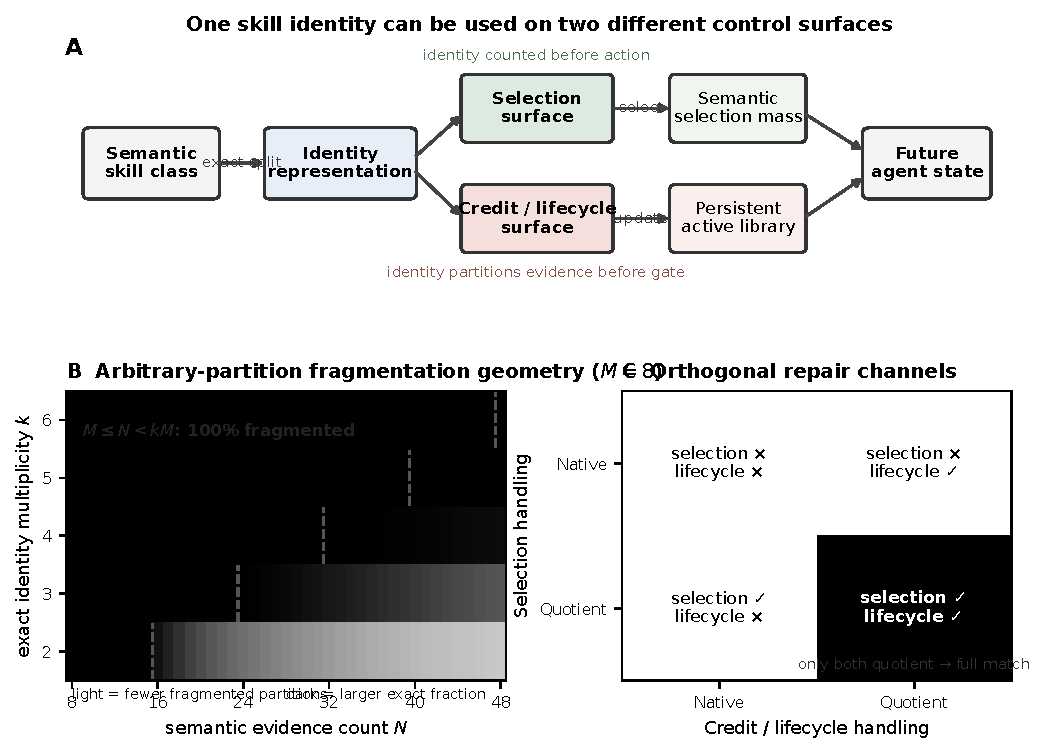
\includegraphics[width=0.99\linewidth]{figures/stri-r2-mechanism-closure.pdf}
\caption{Mechanism closure. \textbf{A:} exact semantic identity refinement can enter the controller through two different surfaces: immediate selection and persistent credit/lifecycle state. \textbf{B:} in released Skill-SP, identity-local thresholding produces the exact credit-fragmentation window $M\le N<kM$ for retirement-eligible evidence ($M=8$). \textbf{C:} the $2\times2$ intervention separates the channels: quotienting either surface alone leaves the other defect, while quotienting both restores both canonical semantic endpoints.}
\label{fig:mechanism-closure}
\end{figure}

\section{Related Work and Reduction Boundaries}

\paragraph{Self-evolving skill systems.}
Skill-SP co-evolves task generation and a persistent skill library~\citep{huang2026skill}; SkillRL recursively evolves a skill library alongside reinforcement learning~\citep{xia2026skillrl}; SkillsVote couples skill-linked attribution to evidence-gated updates~\citep{liu2026skillsvote}; and RethinkSkill studies controlled multi-round feedback views with validation-filtered persistent revisions~\citep{liu2026rethinkskill}. These works establish that skill lifecycle and feedback matter. Our identifying intervention is narrower: hold the semantic feedback multiset fixed, change only its partition across exact-semantic identities, and ask whether the persistent lifecycle endpoint changes.

\paragraph{Replication, redundant actions, and quotient structure.}
Strategic replication in bandits shows that duplicate arms can manipulate selection opportunity~\citep{shin2022replication}; action-redundancy work shows that action multiplicity can misrepresent transition diversity~\citep{baram2021redundancy}. These explain the immediate selection channel and are not claimed as R2 novelty. Likewise, homomorphism and abstraction theory provide mature language for when a quotient preserves dynamics~\citep{ravindran2004approximate}. We use quotient commutation only as an organizing criterion. The empirical/theoretical residual is stage-specific: released self-evolving skill state stores evidence per identity and applies a nonlinear lifecycle gate before semantic aggregation, yielding a directly testable multiplicity/evidence phase boundary.

\paragraph{What is deliberately not claimed.}
Identity fragmentation is already known to bias inference when observations from one underlying entity are split across identifiers~\citep{lin2022identityfragmentation}; generic path dependence and representation-dependent learning are also broader phenomena. Our claim is not that fragmentation exists in the abstract. It is that a released self-evolving skill lifecycle instantiates a particular \emph{partition-before-gate} mechanism: the same skill identity is an action handle and a persistent credit/lifecycle key, so exact semantic refinement can change future action availability even when the post-selection semantic feedback multiset is fixed. The identifying contribution is the stage localization, exact phase law, orthogonal intervention, and persistent-state consequence---not generic identifier fragmentation.

\begin{table}[t]
\centering
\caption{Closest-work reduction boundary. Selection-side redundancy is inherited; R2's identifying intervention fixes post-selection semantic feedback and changes only its exact identity partition.}
\label{tab:reduction}
\small
\setlength{\tabcolsep}{4pt}
\begin{tabular}{p{0.25\linewidth}p{0.67\linewidth}}
\toprule
Neighbor & What is absorbed, and what remains to test\\
\midrule
Strategic replication~\citep{shin2022replication} & Duplicate arms can change selection opportunity; R2 removes selection and still changes persistent lifecycle under fixed feedback.\\
Action redundancy~\citep{baram2021redundancy} & Equivalent actions distort action-level control; R2 isolates identity-keyed evidence containers and future active-library state after action.\\
Identity fragmentation~\citep{lin2022identityfragmentation} & Fragmented identifiers can bias inference; R2 tests partition-before-lifecycle-gate noncommutation, an exact phase law, and a quotient-credit intervention.\\
RethinkSkill~\citep{liu2026rethinkskill} & Feedback views and validation shape multi-round revision; R2 holds feedback content fixed and changes identity partition alone.\\
SkillsVote~\citep{liu2026skillsvote} & Skill-linked attribution already governs updates; R2 uses its release only as independent partition-before-updater structural corroboration.\\
\bottomrule
\end{tabular}
\end{table}

\section{Representation-Invariant Skill Evolution}

\subsection{Semantic quotient and two control surfaces}

Let $\ids_t$ be the active skill identities at evolution round $t$, and let $\pi:\ids_t\to\semclass_t$ map identities to semantic classes. An \emph{exact refinement} replaces an identity with multiple members that are equivalent for the semantic object under study; the quotient class $c\in\semclass_t$ is unchanged.

We distinguish two places where an implementation may use identity.

\paragraph{Selection surface.}
Let $p_t(i)$ be the probability or mass assigned to identity $i$. The semantic selection mass is
\begin{equation}
P_t(c)=\sum_{i:\pi(i)=c}p_t(i).
\end{equation}
Exact refinement is selection-invariant when $P_t(c)$ is preserved. For partial-overlap skill supports, Section~\ref{sec:selection-geometry} generalizes this question beyond exact clones.

\paragraph{Credit/lifecycle surface.}
After a task has produced feedback, identity $i$ stores persistent sufficient state $s_{t,i}\in\mathcal{S}$, with semantic aggregation operator $\agg$. For class $c$ define
\begin{equation}
S_{t,c}=\mathop{\agg}_{i:\pi(i)=c}s_{t,i}.
\end{equation}
Let $g:\mathcal{S}\to\{0,1\}$ be a lifecycle predicate, where $g(s)=1$ denotes retirement in the running example. If a semantic class disappears only when all refined identities retire, native class retirement is $\bigwedge_i g(s_i)$, whereas quotient-credit applies $g$ after semantic aggregation.

\paragraph{Credit-invariance criterion.}
For an exact refinement to be lifecycle-invariant at this gate, the two orders must agree:
\begin{equation}
\label{eq:credit-commute}
g\!\left(\mathop{\agg}_{i:\pi(i)=c}s_i\right)
=\bigwedge_{i:\pi(i)=c}g(s_i).
\end{equation}
Equation~\ref{eq:credit-commute} is not presented as a new abstract quotient theorem. It is an audit condition that exposes where a concrete released update fails to descend to semantic classes.

\subsection{Threshold credit fragmentation}

Consider additive evidence count and a per-identity gate that requires at least $M$ retirement-eligible observations. Let $N$ such observations belong to one semantic class and let $(n_1,\ldots,n_k)$ be \emph{any} weak partition across $k$ exact identities, with $\sum_j n_j=N$.

\paragraph{Proposition 1 (guaranteed fragmentation region).}
Canonical or quotient-credit evolution retires the class iff $N\ge M$, while native evolution retires the full class iff $\min_j n_j\ge M$. Hence for every $k$-way partition,
\begin{equation}
\label{eq:phase-window}
M\le N<kM
\end{equation}
implies fragmentation: aggregate class evidence passes the gate, but at least one identity bucket must remain below $M$. A balanced partition is therefore the \emph{best case} for native recovery, attaining the earliest possible full-retirement boundary $N=kM$ and lag $(k-1)M$.

\paragraph{Partition-dependent tail.}
For $N\ge kM$, invariance becomes allocation-dependent rather than automatic. Among all ordered weak compositions of $N$ into $k$ identities, the exact fraction that remain fragmented is
\begin{equation}
\label{eq:partition-fraction}
F(N,k,M)=1-\frac{\binom{N-kM+k-1}{k-1}}{\binom{N+k-1}{k-1}},
\end{equation}
with $F=1$ throughout Eq.~\ref{eq:phase-window}. We use this combinatorial fraction only to characterize partition geometry; it is not a model of endogenous Skill-SP evidence allocation or prevalence.

\paragraph{Corollary 1 (general gate).}
For identity-local evidence states $(s_1,\ldots,s_k)$ under any mergeable sufficient statistic, a representation defect occurs exactly when the aggregate class state passes the lifecycle gate while at least one identity-local state fails it:
\[
g(s_1\agg\cdots\agg s_k)=1
\quad\text{and}\quad
\exists j:\ g(s_j)=0.
\]
Thus additive statistics alone do not guarantee invariance: nonlinearity enters through applying the lifecycle decision \emph{before} semantic aggregation. Proposition~1 is the threshold-gate specialization that yields a closed-form guaranteed region and a partition-dependent tail in the released Skill-SP mechanism.

The result is elementary by design. Its role is to convert a qualitative mechanism into an ex-ante phase prediction and to expose the exact ordering operation that an intervention must change.

\section{Released Mechanism Realization in Skill-SP}

\subsection{First-party state and update path}

We pin the Skill-SP author release and inspect the actual self-play update path~\citep{huang2026skill}. The released library stores per-ID statistics including attempts and average predicted difficulty; the official loop updates these statistics from skill-linked records and then calls \texttt{prune\_easy\_skills}. The default gate uses $M=8$, average $\hat p$ threshold $0.75$, and too-easy-rate threshold $0.6$. The resulting active library persists into later self-play iterations. Thus identity is concretely both a selectable package and a persistent lifecycle key.

\subsection{P0: fixed-feedback post-selection counterfactual}

To isolate credit from selection, we execute no task selection or retrieval. We externally provide eight identical semantic feedback records with $\hat p=0.9$ to the same released update/pruning functions. Content, support, feedback values, update code, and gate thresholds are fixed.

The canonical representation contains one focal identity plus one background skill. The exact-refinement arm replaces the focal skill with two exact semantic identities and assigns the same eight records alternately. The quotient-credit arm retains the refined interpretation but aggregates the class evidence onto one representative before applying the same released update/gate, then projects the class lifecycle decision back to the refined members.

The results are deterministic: canonical attempts are $8$ and the focal class retires; native split attempts are $(4,4)$ and the class stays active; quotient-credit returns to $8$ and retires the class. The semantic feedback hash is identical across arms. After the update, the native split leaves nonzero future focal sampling mass while canonical and quotient-credit leave none. This is the persistent state transition that selection-only explanations cannot express.

\subsection{P1: phase diagram}

We next sweep $k=1,\ldots,6$, $N=0,\ldots,48$, and $\hat p\in\{0.1,0.5,0.9\}$ through the released controller, producing 882 cells. The two lower-score regimes never retire unexpectedly. In the retirement-eligible $\hat p=0.9$ regime, balanced allocation gives observed first full-retirement boundaries
\[
8,16,24,32,40,48
\]
for $k=1,\ldots,6$, exactly matching the best-case boundary $kM$. Across the entire grid the analytic prediction has zero mismatches. We then independently count all weak evidence compositions for $k=2,\ldots,6$ and $N=8,\ldots,48$ (205 cells) using dynamic programming and compare with Eq.~\ref{eq:partition-fraction}; there are zero count/formula mismatches and every partition in $M\le N<kM$ fragments. At the first tail point $N=kM$, the combinatorial fragmentation fractions for $k=2,3,4,5,6$ are $0.941$, $0.997$, $0.99985$, $0.999993$, and $>0.999999$, respectively. These are geometry summaries under uniform counting of weak compositions, not empirical frequency estimates.

\begin{table}[t]
\centering
\caption{Best-case balanced retirement boundary in released Skill-SP at $M=8$. Proposition~1 is stronger: every partition fragments for $8\le N<8k$; beyond $8k$, fragmentation becomes partition-dependent.}
\label{tab:phase}
\small
\setlength{\tabcolsep}{5pt}
\begin{tabular}{rrrrrrr}
\toprule
$k$ & 1 & 2 & 3 & 4 & 5 & 6\\
\midrule
Native first retirement $N$ & 8 & 16 & 24 & 32 & 40 & 48\\
Lag vs. canonical & 0 & 8 & 16 & 24 & 32 & 40\\
\bottomrule
\end{tabular}
\end{table}

\section{Two-Channel Mechanism Decomposition}

A full representation-invariance account must distinguish the immediate selection surface from the persistent credit surface. We therefore construct a factorial controller counterfactual on one focal semantic class and one background class.

The canonical reference has focal semantic selection probability $1/2$ and, after eight retirement-eligible records, a retired focal class. Exact split2 under native identity normalization raises focal semantic selection to $2/3$. Independently, native per-ID credit splits the eight records $4+4$ and fails to retire the class.

\begin{table}[t]
\centering
\caption{Two-channel intervention on an exact two-way refinement. The canonical reference is semantic selection $1/2$ and retired after eight records. Repairing either identity surface alone leaves the other defect.}
\label{tab:2x2}
\small
\setlength{\tabcolsep}{4pt}
\begin{tabular}{llccc}
\toprule
Selection & Credit & Focal mass & Retired? & Both match?\\
\midrule
Native & Native & $2/3$ & No & No\\
Native & Quotient & $2/3$ & Yes & No\\
Quotient & Native & $1/2$ & No & No\\
Quotient & Quotient & $1/2$ & Yes & \textbf{Yes}\\
\bottomrule
\end{tabular}
\end{table}

Table~\ref{tab:2x2} gives the closure intervention. Quotient selection alone restores the canonical selection mass but leaves the lifecycle defect. Quotient credit alone restores retirement but leaves duplicated selection mass. Applying both restores both frozen semantic endpoints. We therefore treat selection duplication and credit fragmentation as two orthogonal identity channels, rather than folding every representation effect into one generic ``taxonomy bias.''

\section{The General Selection Channel}
\label{sec:selection-geometry}

Exact identity replication is not the only way selection can depend on representation. With partially overlapping skills, a semantic target may be impossible to realize by any nonnegative package weighting even after exact clones are quotiented. Let $A\in\{0,1\}^{n\times m}$ be a frozen task--package support matrix, $w\ge0$ package mass, and $q>0$ a representation-independent target. Package control induces semantic exposure $Aw$. We retain the target-realizability certificate
\begin{equation}
\Rstar(A;q)=\min_{w\ge0,t\ge1}\{t:q\le Aw\le tq\}.
\end{equation}
Then $\Rstar=1$ iff the target lies in the nonnegative support cone; $\Rstar>1$ rules out every same-information controller whose action is still package mass $w$.

This channel is intentionally secondary in R2: its job is to generalize selection-side representation failure beyond exact replication. On Skill-SP Level-1, neutral $\Rstar=2$ on full, calibration, and tool-disjoint heldout matrices. Uniform package mass already attains the exact worst-case optimum, and an eight-fold leave-one-tool-out audit remains at worst-case ratio 2 for uniform and exact $\Rstar$ weights; NNLS reaches 6.10 in the worst fold. In contrast, Level-3 has $\Rstar=1$, and a logical compiler domain has 127/128 multi-membership yet $\Rstar=1$. Thus overlap prevalence is not the mechanism; target realizability is.

\begin{table}[t]
\centering
\caption{Selection-side realizability. High overlap is neither necessary nor sufficient for a residual.}
\label{tab:selection-boundary}
\small
\setlength{\tabcolsep}{4pt}
\begin{tabular}{lrrrl}
\toprule
Regime & Covered & Multi & $\Rstar$ & Outcome\\
\midrule
Skill-SP Level-1 & 314 & 183 & 2.0 & Residual\\
L1 heldout & 52 & 38 & 2.0 & Residual\\
Skill-SP Level-3 & 34 & 0 & 1.0 & Equalizable\\
Logical compiler & 128 & 127 & 1.0 & Equalizable\\
\bottomrule
\end{tabular}
\end{table}

\section{Cross-System Structure and Boundaries}

\subsection{SkillsVote: independent partition-before-update structure}

SkillsVote provides an independent released lifecycle design~\citep{liu2026skillsvote}. Its feedback-to-evolution transformation groups modifiable subtasks by \texttt{skill\_linked}; each identity bucket becomes a separate edit request. The updater iterates over these requests, targets the corresponding persistent working-skill directory, and copies successful edits back to that directory. Its evolution prompt also asks multiple subtasks supporting one improvement to be consolidated within a request.

We execute only this deterministic request-construction path. We create eight feedback records with identical non-identity semantic fields. With all records linked to one focal identity, the release creates one edit request containing eight records. Relinking four records to each of two exact semantic identities creates two edit requests containing four records each. Mapping the two identities back to one semantic quotient restores one eight-record request. The semantic payload hash after removing \texttt{skill\_linked} is identical across all arms.

This corroborates the architecture-level mechanism---identity partitions evidence before the updater sees it---but it does not replicate Skill-SP's lifecycle phase law. SkillsVote's downstream edit is model-based, and we do not execute it here.

\begin{table}[t]
\centering
\caption{Cross-system identity partition before updating. SkillsVote numbers are request topology only; no updater model is called.}
\label{tab:crosssystem}
\small
\begin{tabular}{llll}
\toprule
System/arm & Semantic evidence & Identity buckets & Update contexts\\
\midrule
Skill-SP canonical & 8 records & 1 & 1 bucket, retires\\
Skill-SP split2 & 8 records & 2 $(4+4)$ & 2 buckets, active\\
SkillsVote canonical & 8 records & 1 & 1 request $(8)$\\
SkillsVote split2 & 8 records & 2 $(4+4)$ & 2 requests $(4,4)$\\
SkillsVote quotient & 8 records & 1 semantic class & 1 request $(8)$\\
\bottomrule
\end{tabular}
\end{table}

\subsection{RethinkSkill: a strong negative structural control}

RethinkSkill studies controlled multi-round feedback dynamics with validation-filtered persistent skill revision~\citep{liu2026rethinkskill}. It is therefore a stronger neighbor than a static router. However, its released primary evolution state maintains one current skill, candidates, and a validation gate rather than parallel exchangeable identities with separate evidence buckets. This difference matters for identification: RethinkSkill shows that feedback composition and validation shape evolution, while our counterfactual holds feedback content fixed and varies only exact identity partition before a persistent gate.

\subsection{Natural prevalence remains unresolved}

The Skill-SP mechanism is not an invented toy update: the released loop writes runtime \texttt{skill\_library/skills.json}, updates identity-local statistics before pruning, uses default $M=8$, runs five self-play iterations by default, and targets 8000 total solver records per collection. But runtime \texttt{skills.json} is gitignored and the public release contains no evolved library or retired ledger; three pinned local release mirrors likewise contain no evolved runtime state. We can therefore support mechanism existence and trigger-opportunity plausibility, not the empirical frequency with which endogenous training enters the fragmentation window.

\subsection{Behavior: one manifestation, one binding STOP}

AutoSkill supplies a bounded downstream manifestation~\citep{yang2026autoskill}. In one frozen P19 five-skill library, an exact four-way identity split crowds out a post-checkout skill; the mechanical behavior appears in 6/6 original, 0/6 split, 3/3 ID-placebo, and 3/3 quotient runs (one-sided Fisher $p=0.00108$). Under the split representation, adding the crowded-out post-checkout skill back restores the behavior in 3/3 fresh runs versus 0/3 for a matched cleanup add-back (exact one-sided Fisher $=1/20$). This demonstrates one representation-to-retrieval-to-executed-behavior chain.

We then attempted an outcome-blind heldout replication and stopped it under a frozen gate. Retrieval-only qualification succeeded on 9/9 units. SHA-256 ranking selected two units from different scenarios/positions before behavior was observed. Across 8/8 valid A/B/C/D fresh executions, neither met the preregistered split-specific action-signature criterion: one had identical signatures in all four arms, and the other had native, split, and ID-placebo agreement but a differing quotient control. No repeat-2 or remaining-seven expansion was authorized. Hence retrieval sensitivity is not sufficient for task-general behavioral propagation.

\section{Discussion}

The combined evidence suggests a narrower and more useful interpretation than ``skill names matter.'' A named skill can occupy two distinct coordinates in a self-evolving controller. The \emph{selection coordinate} determines how much immediate semantic opportunity the class receives; exact duplication and partial-overlap support geometry can distort that mass. The \emph{credit coordinate} determines where post-selection evidence accumulates and which persistent object is updated or retired. When a nonlinear lifecycle gate is applied before semantically equivalent evidence is recombined, exact refinement can change the future active library even though the feedback stream is unchanged.

This separation changes the repair logic. A duplication-proof sampler does not repair identity-local credit. Conversely, aggregating credit at the semantic quotient does not correct duplicated selection mass. The $2\times2$ intervention shows that the corresponding quotient interventions are separately necessary for their frozen endpoints and jointly restore both endpoints in the released Skill-SP realization. This is a mechanism-level repair, not a utility claim: we do not show that quotienting either surface improves downstream task performance.

The broader design principle is therefore conditional. If skill identity is intended to be representational rather than semantic, every persistent control surface that consumes identity should be audited for quotient consistency. For selection under partial overlap, $\Rstar$ asks whether the desired semantic target is representable by the package action basis at all. For credit/lifecycle, Eq.~\ref{eq:credit-commute} asks whether evidence aggregation and the lifecycle gate commute. A system can pass one audit and fail the other.

\paragraph{Limitations.}
The exact phase law is established for one released deterministic lifecycle gate; SkillsVote supplies structural corroboration but not a second phase-law replication. Endogenous Skill-SP prevalence is unresolved because evolved runtime state is not released. The AutoSkill heldout STOP prevents task-general behavioral claims. We establish no population utility, safety, longitudinal regret, or universal self-evolution guarantee. Generic quotient theory, action redundancy, strategic replication, and generic identity fragmentation are not claimed as novel.

\paragraph{Takeaway.}
A self-evolving skill identity can be both an action handle and a learning-state handle. Exact semantic refinement is harmless only when the system is invariant at both surfaces. In released Skill-SP, it is not: selection mass and post-selection credit fail through different mechanisms. Separating those mechanisms yields an exact phase prediction, a two-factor intervention, and a concrete criterion for designing representation-invariant skill evolution.
